%-------------------------------------------------------------------------------------------------------
%-------------------------------------------------------------------------------------------------------
% Sec & Label

\section{Simulation Analysis}
\label{sec:simulation}


%-------------------------------------------------------------------------------------------------------
%-------------------------------------------------------------------------------------------------------
% Intro

In this section, Circuit T4 is reproduced with the help of Ngspice.

Ngspice is a simulator for eletronic circuits that can output a variety of results.
This emulator computes the voltages in every node, as well as the potential difference
between two given nodes. Apart from that, the group made use of the command
{\em .options savecurrents} which also enables the use of the currents that pass
through all branches. Moreover, function to help determine the maximum and interception
of the plots were also used.

Firstly, the outcome of the simulation is shown, as well as a brief explanation
on how it was achived. Afterwards, a comparison is done between those values and
the ones attained in Section \ref{sec:analysis}.



%-----------------------------------------------------------------------
%-----------------------------------------------------------------------
% 			     Results - subsec
% ----------------------------------------------------------------------
% ----------------------------------------------------------------------

\subsection{Simulated results}
\label{subsec:sim_res}

In this laboratory assignament, the Ngspice script made use of the sames values considered for
the Octave script.

Figure \ref{fig:Vout} displays $v_{out}$. This voltage signal has no visible distortion of the input sine waves.

\begin{figure}[ht]
	\centering
	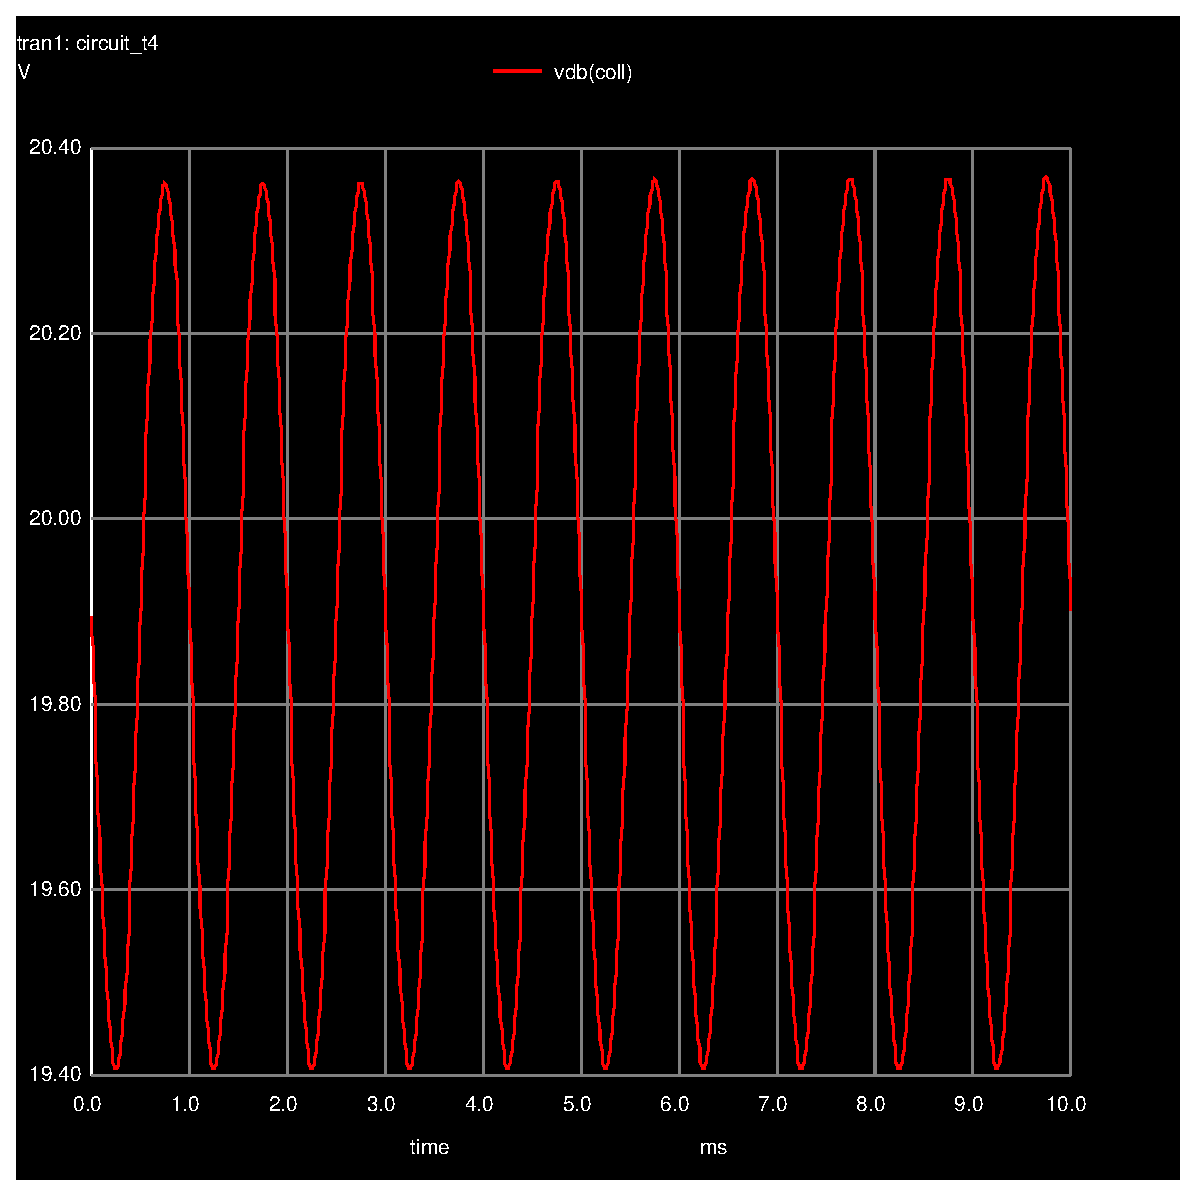
\includegraphics[width=0.6\linewidth]{vo1.eps}
	\caption{$v_{out}$}
\label{fig:Vout}
\end{figure}

Figure \ref{fig:VcollDB} shows $v_{coll}$.

\begin{figure}[ht]
	\centering
	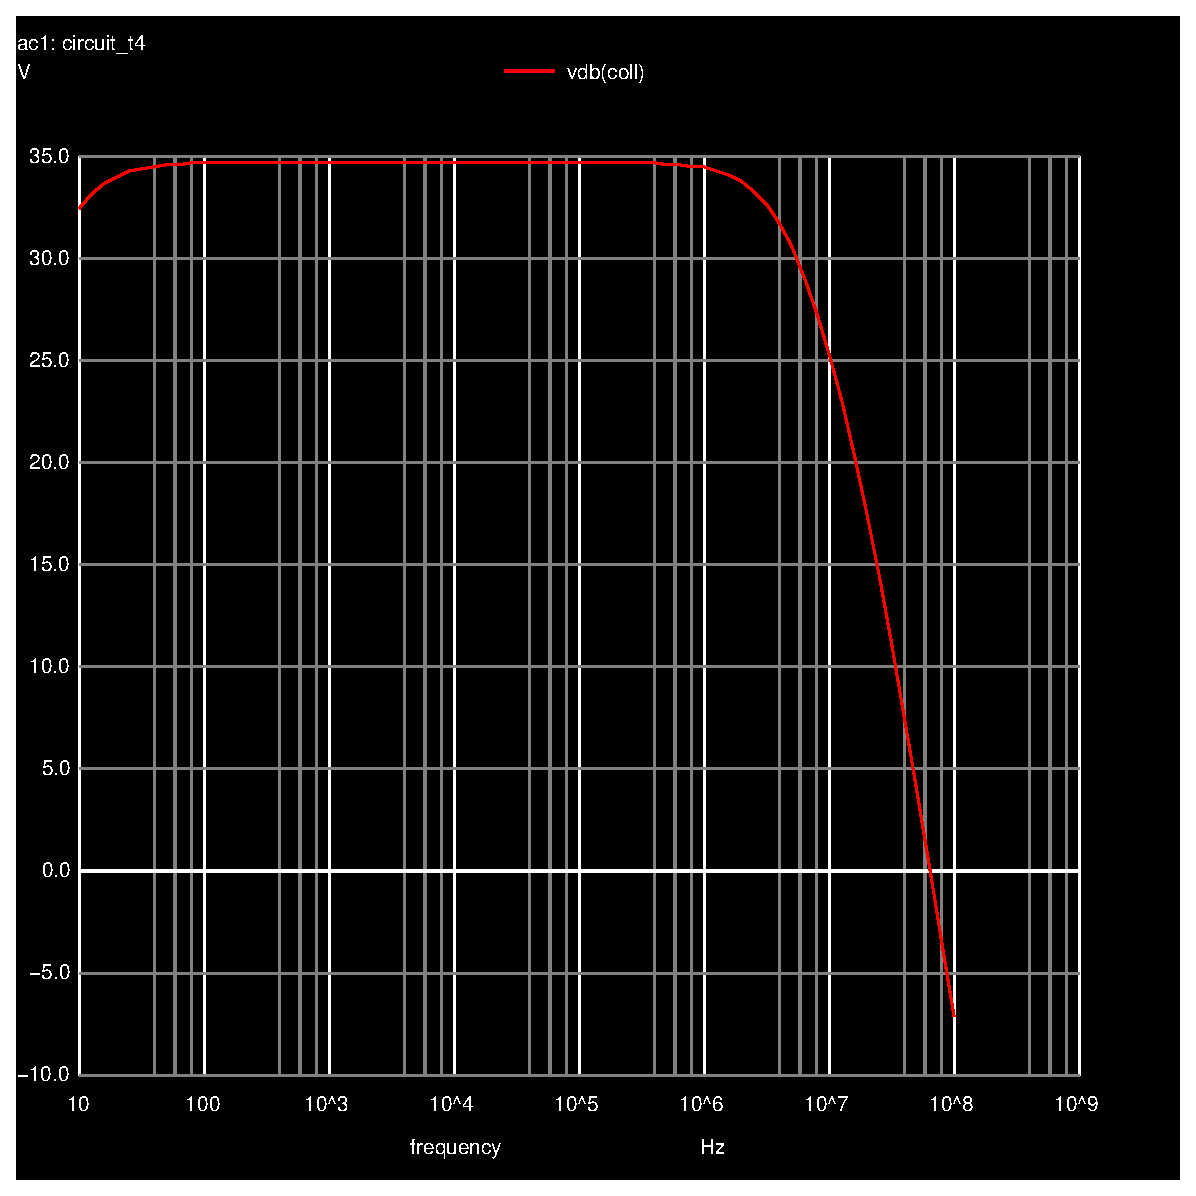
\includegraphics[width=0.6\linewidth]{vo1f.eps}
	\caption{$v_{coll}$ in dB}
\label{fig:VcollDB}
\end{figure}

Figure \ref{fig:Vout} displays $v_{out}$.

\begin{figure}[ht]
	\centering
	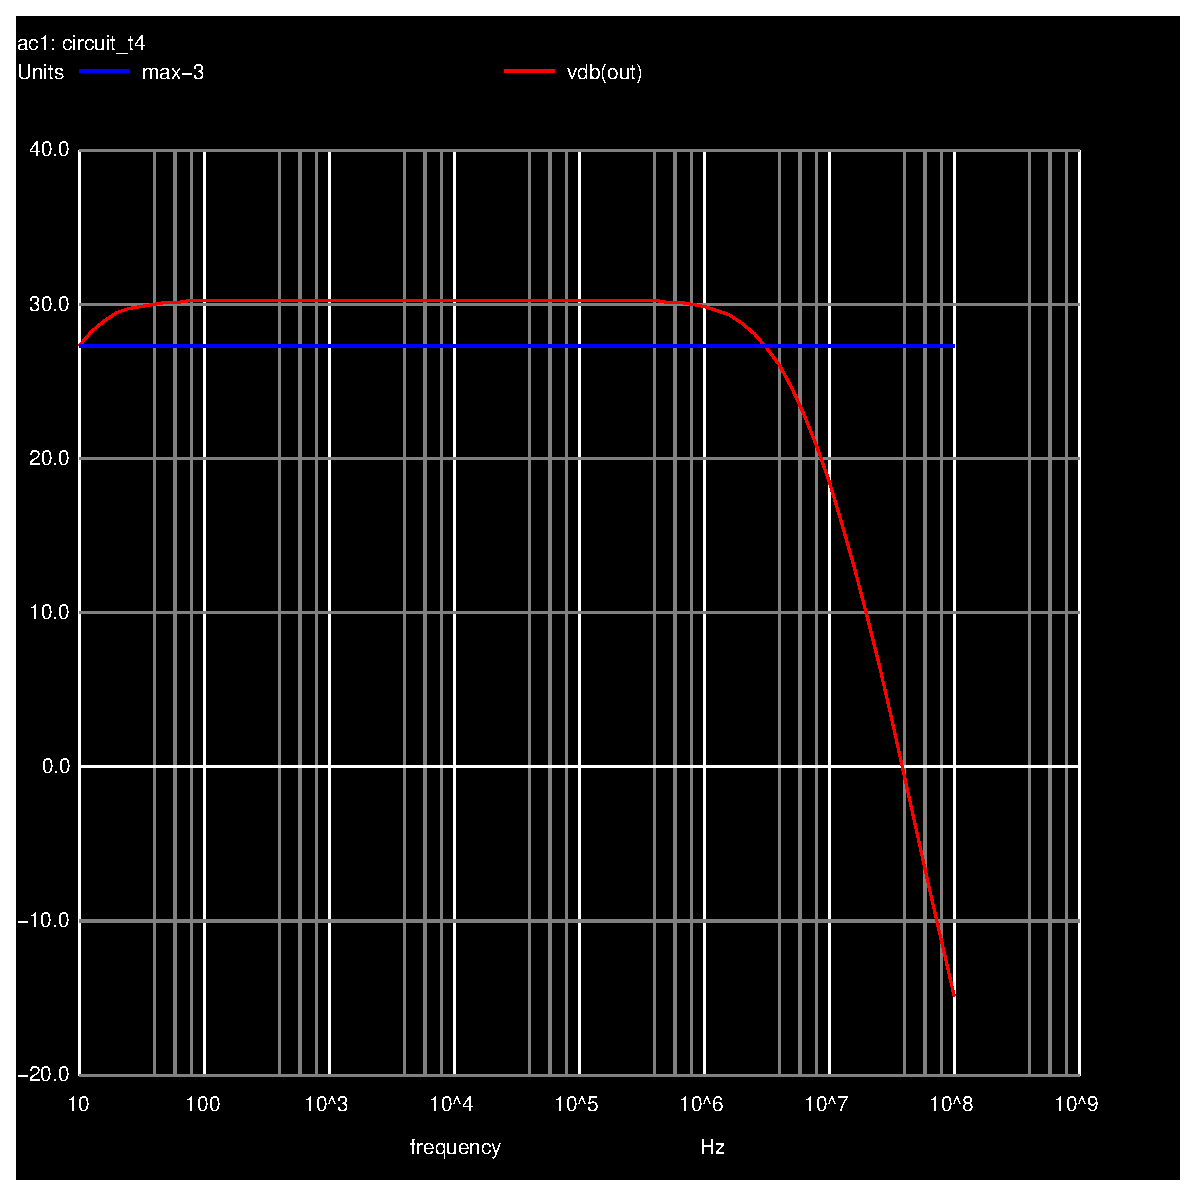
\includegraphics[width=0.6\linewidth]{vo2f.eps}
	\caption{$v_{out}$ in dB}
\label{fig:VoutDB}
\end{figure}

Table \ref{tab:op_sim} shows important values to make the BJTs operate in the F.A.R.

\begin{table}[ht]
	\centering
	\begin{tabular}{|l|r|}
		\hline    
		{\bf Name} & {\bf Value} \\ \hline
    		v(coll) & 1.005359e+01\\ \hline
v(emit) & 1.117079e+00\\ \hline
v(emit2) & 1.086574e+01\\ \hline
v(emit2)-v(coll) & 8.121456e-01\\ \hline
v(coll)-v(base) & 8.244599e+00\\ \hline
v(coll)-v(emit) & 8.936511e+00\\ \hline
v(base)-v(emit) & 6.919123e-01\\ \hline

	\end{tabular}
	
	\caption{Checking values for F.A.R.}
    
\label{tab:op_sim}
\end{table}

Table \ref{tab:imp_sim} dislpays the total impedances od the circuit (In and Out).

\begin{table}[ht]
	\centering
	\begin{tabular}{|l|r|}
		\hline    
		{\bf Name} & {\bf Value[Ohm]} \\ \hline
    		Zin & 9.9022 + 0.00223195 j\\ \hline
Abs(Zin) & 9.9022\\ \hline

    		Zout & 522.442 + -316.233 j\\ \hline
Abs(Zout) & 610.695\\ \hline

	\end{tabular}
	
	\caption{Total impedance values from Ngspice.}
    
\label{tab:imp_sim}
\end{table}

Lastly, the group also used Ngspice to compute the Merit. Table \ref{tab:merit} shows all the 
values necessary to compute the Merit, as well as the Merit itself.

\begin{table}[ht]
	\centering
	\begin{tabular}{|l|r|}
		\hline    
		{\bf Name} & {\bf Value} \\ \hline
    		cost & 1.343451e+04\\ \hline
gain & 1.003168e+02\\ \hline
gaindev & 3.167835e-01\\ \hline
centralfreq & 8.476811e+02\\ \hline
centralfreqdev & 1.523189e+02\\ \hline
 ---------- & -------------------- \\ \hline
merit & 4.876656e-07\\ \hline

	\end{tabular}
	
	\caption{Merit and other variables.}
    
\label{tab:merit}
\end{table}


%-----------------------------------------------------------------------
%-----------------------------------------------------------------------
% 			     Analise - subsec
% ----------------------------------------------------------------------
% ----------------------------------------------------------------------

\subsection{Simulated analysis}
\label{subsec:sim_an}

\subsubsection{Coupling Capacitors}

The purpose of the coupling capacitors on the audio amplifier circuit is to eliminate the DC component of a signal and only pass the AC component, which in the case of an audio amplifier is what carries the sound information.

This arrangement of capacitors is normally used to link/couple (that’s where it´s name comes from) only the AC signal of one circuit to another.

\subsubsection{Bypass capacitor}

A bypass capacitor’s purpose is to remove the AC component of a signal by shorting it to ground.
For this to work, the bypass is placed in parallel with a resistance. Since the capacitor’s impedance follows the equation $|Z_c|=1/wC$ , for DC signals ($w=0$) the impedance is infinite and so all the current flows trough the resistor. When the frequency increases, the capacitor’s impedance decreases and so a larger part of the signal passes trough the capacitor directly to ground. This way, the DC signal is the main contributor to the voltage difference between the components, while the AC signal directed to ground without any resistance.

In our application, the bypass capacitor is used to allow to have the resistance $R_E$ without degenerating the gain. The resistance $R_E$ adds temperature stabilization and removes the temperature dependency of the gain in the circuit has the drawback of decreasing the AC gain of the amplifier. For this purpose, only the DC component needs to be affected by the resistance $R_E$ and for this reason, the bypass capacitor is used so that higher frequencies are not affected by $R_E$. This way we can achieve the best of temperature stabilization without gain degeneration.

